% Docker Meetup at MfN, 24 April 2018
% Running wikis at the Museum with Docker - past, present and future
% Alvaro Ortiz-Troncoso
% 
% Template:
% see https://en.wikibooks.org/wiki/LaTeX/Presentations
% http://ctan.127001.ovh/macros/latex/contrib/beamer/doc/beameruserguide.pdf

%%% Local Variables:
%%% mode: latex
%%% TeX-master: t
%%% End:
\documentclass[12pt]{beamer}
\usepackage[utf8]{inputenc}
\usepackage{graphicx}
\usepackage{xcolor}
\usepackage[sfdefault]{roboto}

\definecolor{mfn_green}{HTML}{A1BF23}
\definecolor{mfn_blue}{RGB}{0, 153, 187}

%\renewcommand{\sfdefault}{\roboto}
%\renewcommand{\familydefault}{\sfdefault}

\setbeamercolor{title}{fg=black}
\setbeamerfont{title}{series=\bf,size={\fontsize{25}{30}}}

\setbeamerfont{subtitle}{shape=\itshape,size={\fontsize{20}{25}}}
\setbeamerfont{frametitle}{size={\fontsize{18}{22}}}
\setbeamercolor{frametitle}{fg=black}
\setbeamercolor{footline}{fg=gray}
\beamertemplatenavigationsymbolsempty
%\setbeamertemplate{footline}[page number]
\setbeamertemplate{itemize item}{\color{mfn_green}$\blacktriangleright$}
\setbeamertemplate{caption}{\scriptsize\insertcaption}
\setbeamersize{text margin left=5mm,text margin right=7mm}
\setlength\abovecaptionskip{-5pt}
\setbeamertemplate{footline}{
  \mbox{\hspace{1em}\insertshorttitle}
  \newline\smallskip\newline
  \mbox{\hspace{1em}\insertshortauthor \textbar Museum für Naturkunde Berlin – Leibniz-Institut für Evolutions- und Biodiversitätsforschung}
  \newline\smallskip\newline
}

\title{Running wikis at the Museum with Docker}
\subtitle{past, present and future}
\author{Alvaro Ortiz-Troncoso}
\date{Docker Meetup at Museum für Naturkunde Berlin, 2018}
\subject{Computer Science}

\begin{document}

%----------------------------------------------------------------------------------------------%
% 1. Titelseite
{
  \setbeamertemplate{footline}{}
  {
  \logo{
\includegraphics[height=1cm]{mfn_logo_klein.png}\vspace{220pt}}
  \frame{\titlepage}
  }
}
\addtocounter{framenumber}{-1}
%----------------------------------------------------------------------------------------------%
% 2. Das Museum
\begin{frame}
  \frametitle{Das Museum / \textcolor{mfn_green}{The Museum}}
  \begin{figure}
    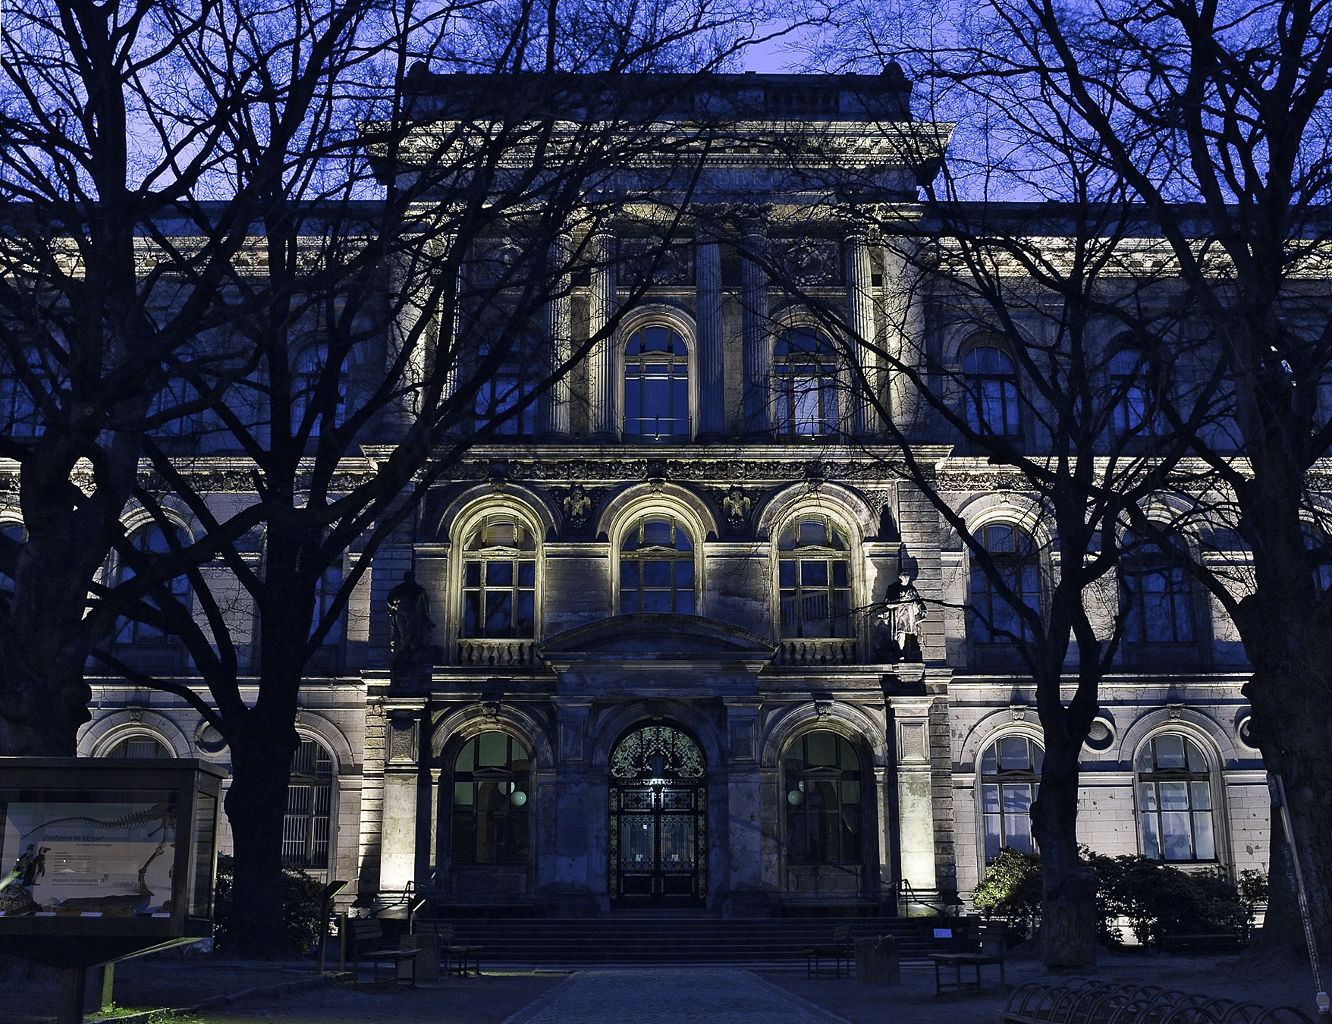
\includegraphics[height=70mm]{Gebaeude_Nacht.jpg}
    \caption{\textcopyright Antje Dittmann, Museum für Naturkunde Berlin, 2009. CC-by-sa}
  \end{figure}
\end{frame}

{\scriptsize
\begin{frame}
  \frametitle{Das Museum / \textcolor{mfn_green}{The Museum}}
  Dieser Vortrag handelt von unserer Erfahrung mit der Kombination von Docker und Wikis am Museum. Zuerst werde ich kurz sprechen über was wir am Museum tun, und über wie wir es tun. Das Museum ist ein sehr dynamisches Umfeld, und hier zu arbeiten ist vielleicht anders, als die meisten Aussenstehenden sich das vorstellen. Danach werde ich über Wikis und Docker sprechen. Ich werde die Gründe durchnehmen, wieso wir uns für Docker entschieden haben, sowohl organisatorisch als auch technisch. Schließlich werde ich über unsere Zukunftspläne sprechen. Besonders darüber freue ich mich über Feedback, Anregungen, Kritik und Ideen.\\
  \bigskip
  \textcolor{mfn_green}{This talk is about our experience with combining Docker and wikis at the Museum. First I'll talk shortly about what we do at the Museum, and how we do it. The Museum is a very dynamic environment, and working here is probably very different from what most people imagine. Then I'll talk about running wikis with Docker. I'll go into the reasons for adopting Docker, both organisational and technical. Finally, I'll talk about plans for the future. Particularly regarding our plans, I'm very interested in hearing your feedback, criticism, and ideas.}
\end{frame}
}
%----------------------------------------------------------------------------------------------%
% 3. Ausstellung
\begin{frame}
  \frametitle{Die Ausstellung / \textcolor{mfn_green}{The exhibition}}
  \begin{figure}
  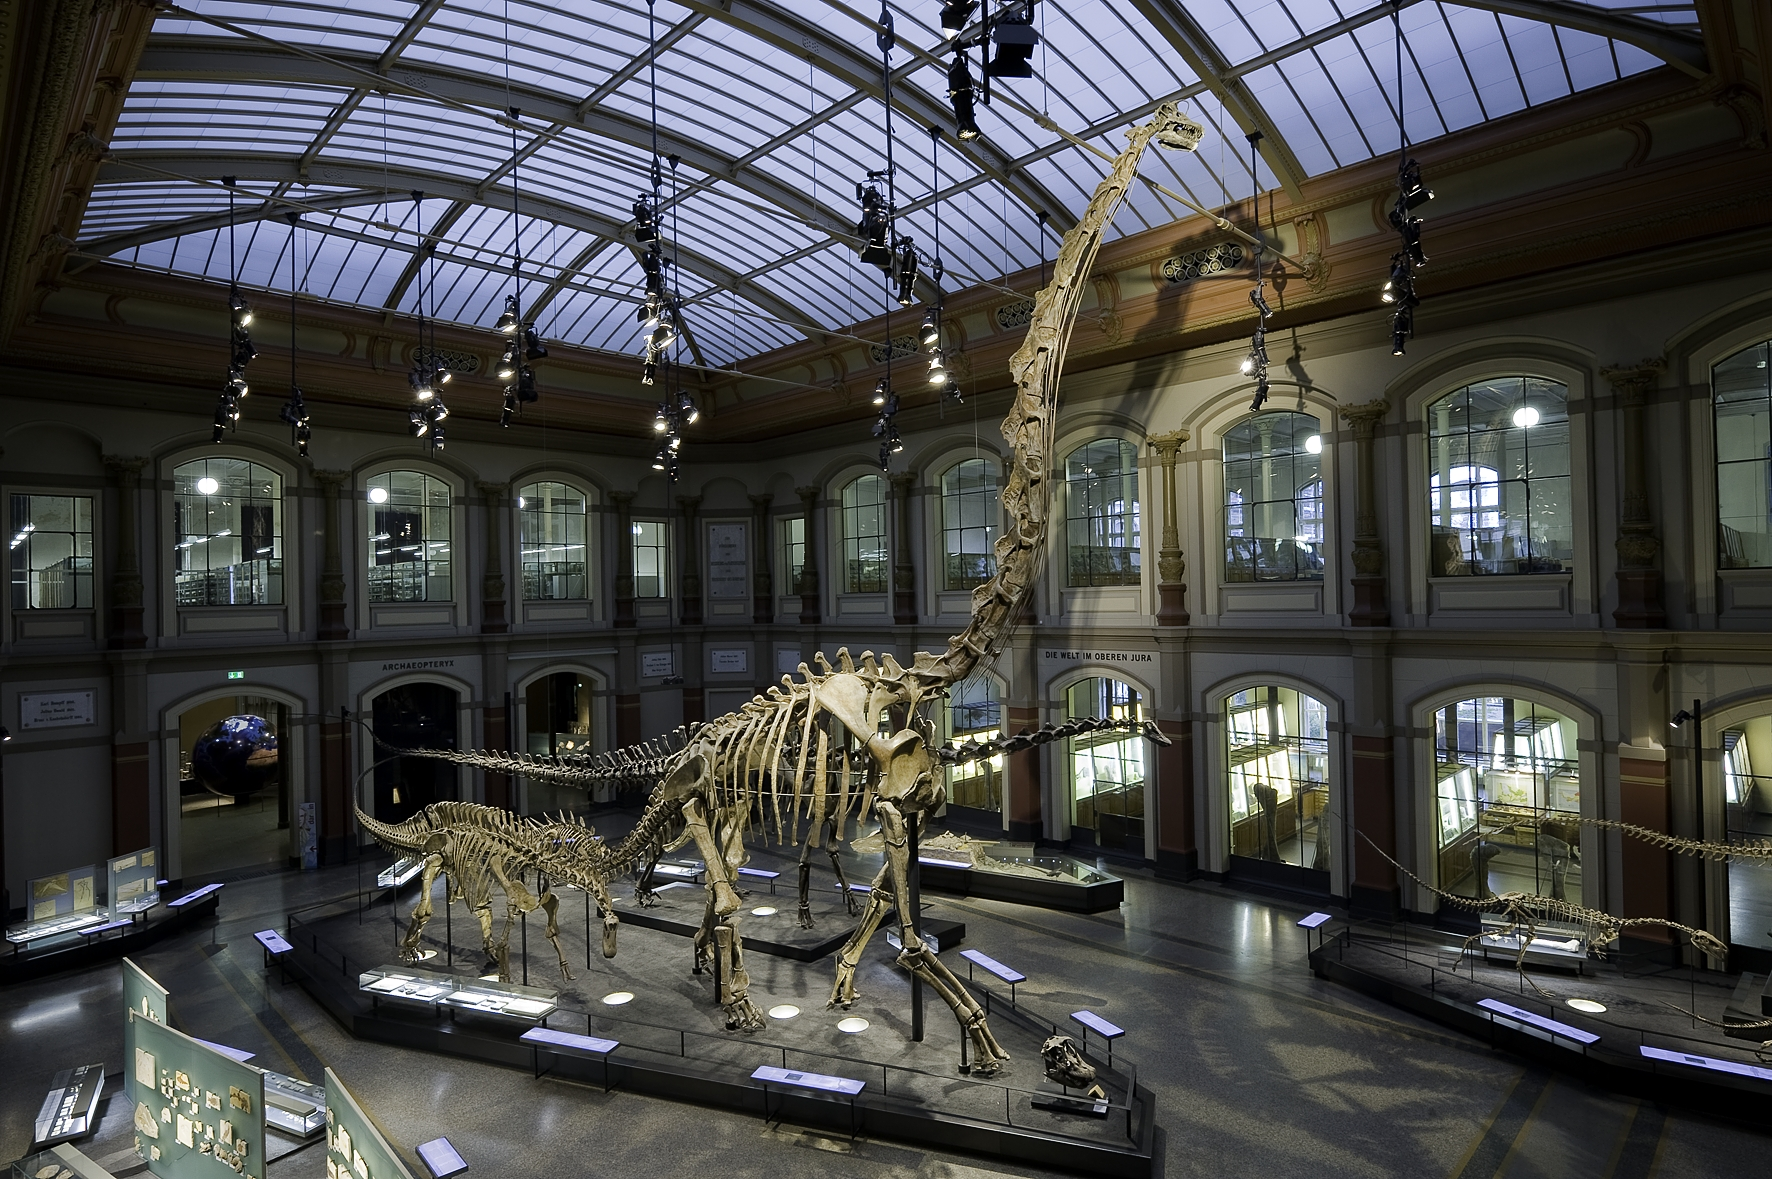
\includegraphics[height=70mm]{Brachiosaurus_02_15cm.jpg}
  \caption{\textcopyright Antje Dittmann, Museum für Naturkunde Berlin, 2009. CC-by-sa}
  \end{figure}
\end{frame}

{\scriptsize
\begin{frame}
  \frametitle{Die Ausstellung / \textcolor{mfn_green}{The exhibition}}
Die meisten Personen denken, dass das Museum und die Ausstellung gleichzusetzen sind. Das entspricht nur zum Teil die Wahrheit. Den Meisten ist es bewusst, dass nicht alles, was das Museum besitzt, ausgestellt werden kann, aber die Menge an Forschung, die hinten den Kulissen betrieben wird, ist den meisten Personen nicht bewusst.\\
  \bigskip
  \textcolor{mfn_green}{Most people think the Museum is the exhibition. This is partly true, but there is much more going on behind the scenes. Of course, many people know that museums cannot display everything they have. But most people are unaware of the amount of research that is carried out on the collection.}
\end{frame}
}
%----------------------------------------------------------------------------------------------%
% 4. Einige Zahlen
\begin{frame}
  \frametitle{ Einige Zahlen / \textcolor{mfn_green}{Some numbers}}

  \begin{itemize}
  \item{Personal: 289, Studenten: 209}
  \item{Publikationen: 222 / Jahr (2016)}
  \item{Aktuell erforschen 51 Projekte die Sammlung}
  \end{itemize}
  
  \begin{itemize}
  \item{\textcolor{mfn_green}{Staff: 289, Students: 209}}
  \item{\textcolor{mfn_green}{Publications 222 / year (2016)}}
  \item{\textcolor{mfn_green}{Currently 51 projects are researching the collection}}
  \end{itemize}
  \bigskip
  \begin{center}\scriptsize{Unsere Wissenschaft / Our Science, DOI: 10.7479/3dwq-8a7g}\end{center}
\end{frame}

{\scriptsize
\begin{frame}
  \frametitle{ Einige Zahlen / \textcolor{mfn_green}{Some numbers}}
  Fast 500 Personen arbeiten im Museum: WissenschaftlerInnen, StudentInnen, Labor TechnikerInnen, EntwicklerInnen und so weiter. Wie in jedem Wissenschaftsinstitut kann die Produktion an der Menge der Publikationen gemessen werden. Mit Publikationen sind hier sowohl wissenschaftliche Artikel in spezialisierten Zeitschriften als Ausstellungskataloge und so weiter gemeint. Zur Zeit sind 51 Forschungsprojekte am Museum aktiv, und erforschen die Sammlung, die Forschung an der Sammlung, die Forschung an der Forschung an der Sammlung...\\
  \bigskip  
  \textcolor{mfn_green}{Almost 500 persons work at the museum, including scientists, students, lab technicians, software developers and so on. As in any science institution, output can be measured by the number of publications. These include science publications but also books and articles in magazines. There are currently 51 projects researching the collection, or researching the scientists working on the collection, on the research on the research on the collection.}
\end{frame}
}
%----------------------------------------------------------------------------------------------%
% 5. Forschungsprojekte
\begin{frame}
  \frametitle{Forschungsprojekte / \textcolor{mfn_green}{Research projects}}
  \begin{figure}
  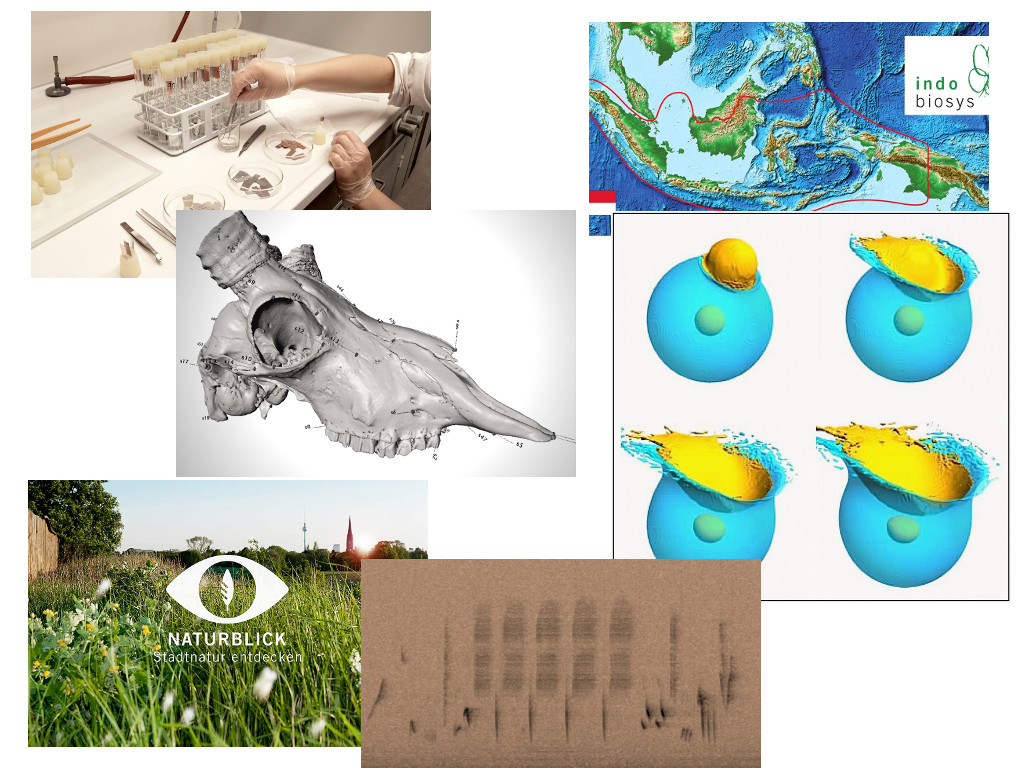
\includegraphics[height=70mm]{Forschung.jpg}
  \caption{https://www.museumfuernaturkunde.berlin/}
  \end{figure}
\end{frame}

{\scriptsize
\begin{frame}
  \frametitle{Forschungsprojekte / \textcolor{mfn_green}{Research projects}}
  Hier sind einige Beispiele von Forschungsprojekte: im Museum sind mehrere Labore untergebracht, wo verschiedene Arten von Forschung betrieben wird, zum Beispiel zu Genetik. Das Museum benutzt 3D-Scanners um die Sammlung zu digitalisieren. Das Museum ist auch in ökologische Projekte involviert, zum Beispiel zur Biodiversitätsforschung in besonders interessante Gebiete. Geologen am Museum erforschen die Folgen von Meteoriteneinschläge und benutzen dazu Computersimulationen. Das Museum hat ein App entwickelt, das bei der Bestimmung von Pflanzen und Vogestimmen helfen kann. Diese sind fast zufällig ausgewählte Projekte auf unsere Webseite.\\
  \bigskip
  \textcolor{mfn_green}{Here are some examples of research projects: the Museum hosts a number of laboratories, where research is carried out in many fields, such as genetics. The Museum is using 3D-scanners to digitise the collection. The Museum is also involved in ecological projects, for example in mapping the biological diversity in specially interesting region. Geologists at the Museum are modelling planetary impacts, and meteorites. The Museum also developed an App, that can be downloaded from the App-Store, that helps to identify birds by song and plants using a mobile phone. These are just a few almost randomly chosen examples of projects on our Website.}
\end{frame}
}
%----------------------------------------------------------------------------------------------%
% 6. Was macht ein Projekt aus?
{
\setbeamercolor{background canvas}{bg=mfn_green}
\setbeamercolor{frametitle}{fg=black}
\begin{frame}
  \frametitle{Was macht ein Projekt aus? \\ \textcolor{white}{What does it take to launch a project?}}
  \begin{figure}
  \includegraphics[height=70mm,trim=4 4 4 4,clip]{Projekt.png}
  \end{figure}
  \bigskip
\end{frame}
}

{\scriptsize
\begin{frame}
  \frametitle{Was macht ein Projekt aus? \\ \textcolor{mfn_green}{What does it take to launch a project?}}
  Einerseits soll das Museum die Sammlung konservieren und kuratieren, für die Ewigkeit. Andererseits, passieren hier all diese aufregende, dynamische Dinge. Das ist möglich, weil wir in Projekten arbeiten. Ein Projekt brauch im Grunde genommen nur 3 Voraussetzungen: Finanzierung, Zeitplan (Projekte haben einen Anfang und ein Ende) und Team. Forschungsteams am Museum bestehen typischerweise aus Wissenschaftler und Mitarbeiter aus verschiedenen Disziplinen, wie zum Beispiel Software-EntwicklerInnen, System-Administratoren, Projektmanagers, Designer, Fotografen, LabortechnikerInnen usw.\\
  \bigskip
  \textcolor{mfn_green}{On the one hand, the Museum is meant to preserve and curate the collection, forever. On the other hand, we do all this exiting, dynamic stuff. This is possible because our work is organised in research projects. A project has 3 basic needs: funding, a time plan (a project has a beginning and an end), and most importantly a team. Research teams at the Museum often include a researcher and collaborators from many different fields, such a software developers, system administrators, management people, designers or photographers, lab technicians and so on.}
\end{frame}
}
%----------------------------------------------------------------------------------------------%
% 7. Kooperation
\begin{frame}
  \frametitle{Kooperation / \textcolor{mfn_green}{Cooperation}}

  \begin{itemize}
  \item{Gemeinsames Verständnis der Projektziele}
  \item{Innerhalb des Zeitrahmens zum Ergebnis kommen}
  \item{Den Kostenrahmen nicht überschreiten - Effizient arbeiten}
  \end{itemize}
  
  \begin{itemize}
  \item{\textcolor{mfn_green}{Common understanding of project goals}}
  \item{\textcolor{mfn_green}{Deliver on time}}
  \item{\textcolor{mfn_green}{Be efficient to finish within budget}}
  \end{itemize}
\end{frame}

{\scriptsize
\begin{frame}
  \frametitle{Kooperation / \textcolor{mfn_green}{Cooperation}}
  Kooperation ist nötig aus mindestens drei Gründe: ein Team, das aus Mitarbeitern mit verschiedenen Hintergründe und Spezialisierungen besteht, muss zu einem gemeinsamen Verständnis kommen, was die Ziele des Projekts sind. Zum Beispiel kann "Erfolg" für einem Wissenschaftler was völlig anderes sein als "Erfolg" für einen Manager. Kooperation ist auch nötig, um das Zeitplan einzuhalten. Jeder, der an einem Projekt gearbeitet hat, weiß, das die Zeit nie reicht. Kooperation ist aber auch nötig, um innerhalb des Kostenrahmens zu bleiben, denn wer kooperiert arbeitet auch effizienter.\\
  \bigskip
  \textcolor{mfn_green}{Cooperation is necessary for at least 3 reasons: a team that is made of persons coming from different fields and specialities, needs to come to a common understanding of what it is they wish to achieve. For example, "success" for a scientist might be something totally different than "success" for a manager. Cooperation is also necessary to deliver on time. As anybody who has worked on a project can tell, there is never enough time. Cooperation is also necessary to work efficiently and deliver within budget.}
\end{frame}
}
%%%%%%%%%%%%%%%
%
% The past
%
%%%%%%%%%%%%%%%

%----------------------------------------------------------------------------------------------%
% 8. In der Vergangenheit
\begin{frame}
  \frametitle{In der Vergangenheit / \textcolor{mfn_green}{In the past}}
  \begin{figure}
    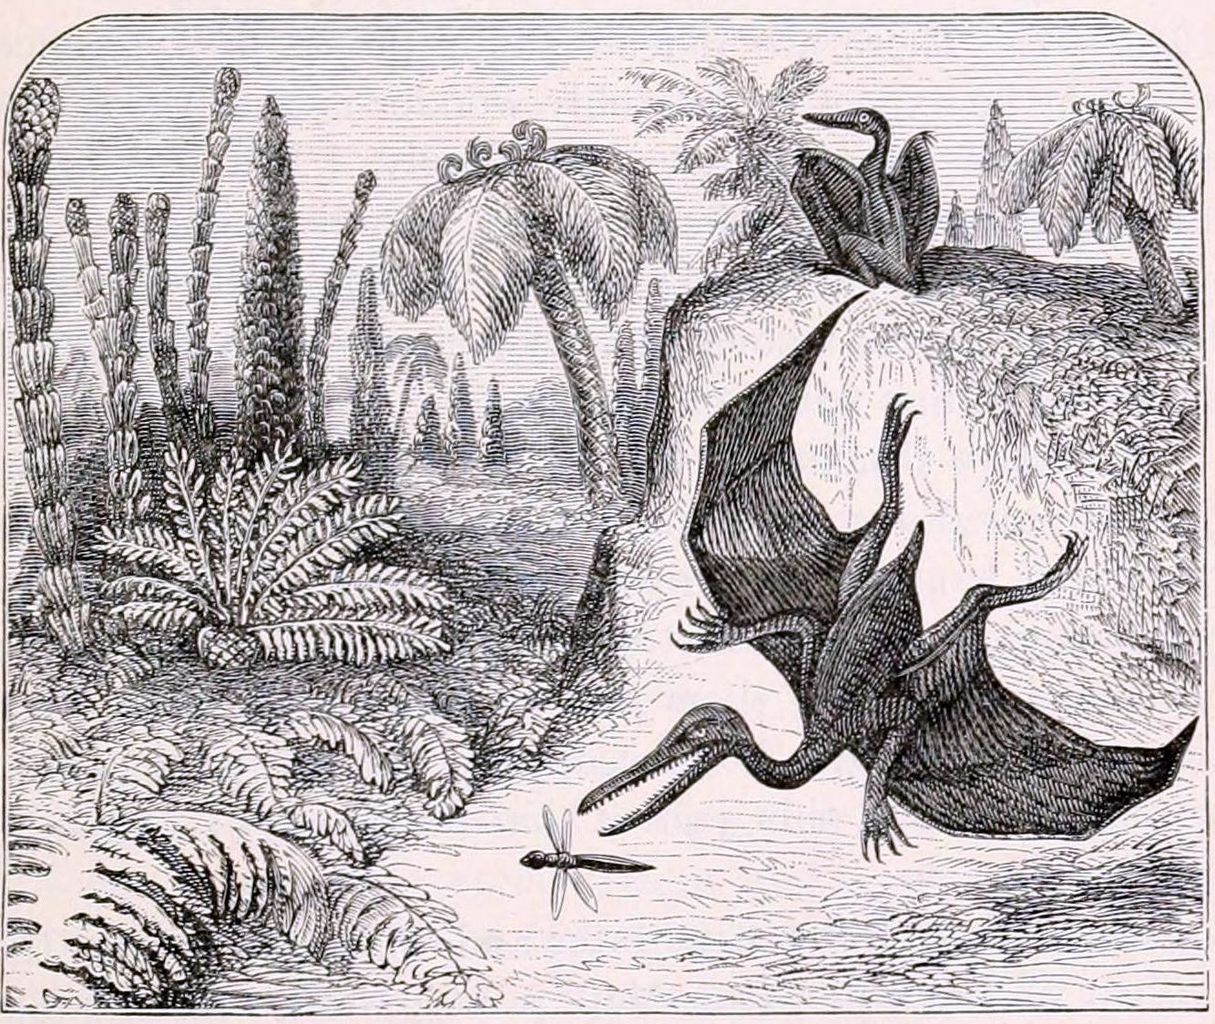
\includegraphics[height=70mm]{Ideal_Landscape_of_a_Prehistoric_Age.jpg}
    \caption{Quackenbos, J.D., 1886. \textit{Illustrated School History of the World}. D. Appleton.}
  \end{figure}
\end{frame}

%----------------------------------------------------------------------------------------------%
% 9. Word .doc Hölle
{
\setbeamercolor{background canvas}{bg=mfn_green}
\setbeamercolor{frametitle}{fg=black}
\begin{frame}
  \frametitle{Word\textsuperscript{\tiny\textregistered} .doc Hölle /
    \textcolor{white}{Word\textsuperscript{\tiny\textregistered} .doc hell}}
  \begin{figure}
  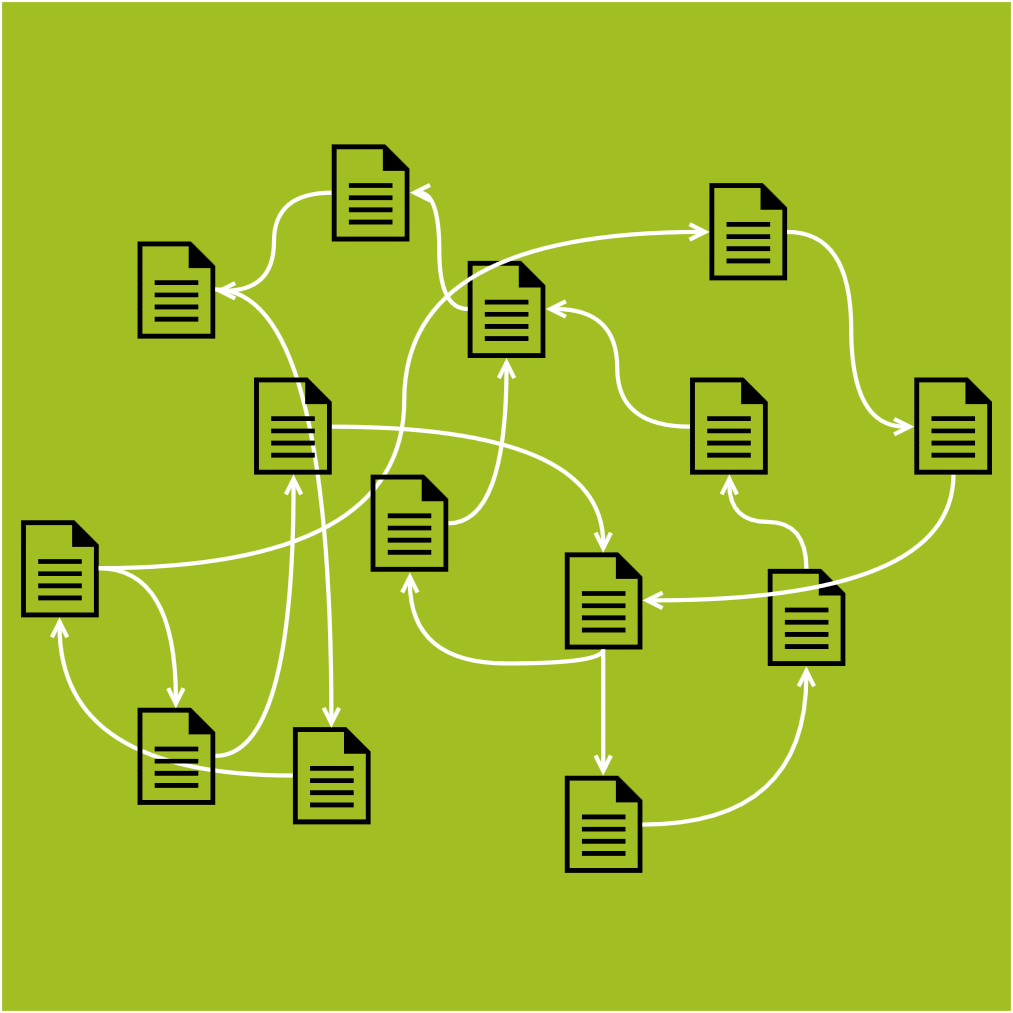
\includegraphics[height=70mm,trim=4 4 4 4,clip]{Docs.png}
  \end{figure}
\end{frame}
}

{\scriptsize
\begin{frame}
  \frametitle{Word\textsuperscript{\tiny\textregistered} .doc Hölle /
    \textcolor{mfn_green}{Word\textsuperscript{\tiny\textregistered} .doc hell}}
Früher war Kooperation durch hin-und-her schicken von Papierunterlagen geprägt. Leider gibt es immer noch viele Personen, die diese Art und Weise eins-zu-eins in die digitale Welt übernommen haben. Eine primitive Art der Kooperation ist, Word Dokumente auf eine gemeinsam benutzte Festplatte zu speichern, und die Adresse des Dokuments an den Projektmitarbeitern per Email zu verschicken. Weil Word keine Kooperationsfunktionen hat, bedeutet es, dass ein Dokument, das von einem Mitarbeiter geöffnet ist, von den anderen nicht bearbeitet werden kann. Weil das sehr oft passiert, ist es Usus geworden, Word Dokumente als Beilage zu Emails zu verschicken, ein Rezept für endgültiges Chaos.\\
  \bigskip
  \textcolor{mfn_green}{In the past, the only way to cooperate was through exchanging paper documents. Unfortunately, many people still think this way, except that Word documents have replaced paper. So a primitive way of cooperating is to place a Word document on a shared drive and to email the documents address to your collaborators. As Word does not support collaboration, this means that a document that is opened for editing by one person cannot be edited by anyone else. As this happens very often, people have taken to sending documents as email attachments, which is a definitive receipt for final chaos.}
\end{frame}
}
%----------------------------------------------------------------------------------------------%
% 10. Nichts gegen Word aber...
\begin{frame}
  \frametitle{Nichts gegen Word\textsuperscript{\tiny\textregistered} aber... \\
    \textcolor{mfn_green}{Absolutely nothing against Word\textsuperscript{\tiny\textregistered}, however, ...}}
  \begin{itemize}
  \item{Keine Versionierung: wer hat die Endfassung?}
  \item{Kein Dokumentverlauf: wer hat was geschrieben?}
  \item{Proprietäre Software: Anbieterabhängigkeit}
  \end{itemize}
  
  \begin{itemize}
  \item{\textcolor{mfn_green}{No versioning: who has the final version}}
  \item{\textcolor{mfn_green}{No document history: who wrote what?}}
  \item{\textcolor{mfn_green}{Proprietary software: vendor lock-in}}
  \end{itemize}
\end{frame}

{\scriptsize
\begin{frame}
  \frametitle{Nichts gegen Word\textsuperscript{\tiny\textregistered} aber... \\
    \textcolor{mfn_green}{Absolutely nothing against Word\textsuperscript{\tiny\textregistered}, however, ...}}
  Obwohl Word ein ziemlich gutes Programm ist, hat es für kooperatives Arbeiten gewisse Nachteile: es gibt keine Möglichkeit herauszufinden, welche der Kopien des Dokuments, die per Email in Umlauf gebracht sind, die endgültige Fassung ist. Oder, wenn es mehrere Fassungen des Dokuments gibt, gibt es keine Möglichkeit, die verschiedenen Fassungen zusammenzufügen. Word bietet keine Möglichkeit zur Verfolgung der Autorschaft des Dokuments oder Teile davon. Autorschaft ist essentiell für ForscherInnen, denn ihre wissenschaftliche Reputation basiert darauf. Ein andere Nachteil von Word ist, dass es sich um proprietäre Software handelt. Das Museum existiert seit 1889, und wird nicht nur uns überleben, sondern mit aller Wahrscheinlichkeit auch Microsoft, und was ist dann?\\
  \bigskip
  \textcolor{mfn_green}{Although Word is quite a good programme, when it comes to cooperation it has some very clear disadvantages: There is no way to know which one of the document copies is the final version, or if there are several versions, there is no way to automatically merge documents. Word does not provide a transparent mechanism to follow who wrote which part of a document. Authorship is very important for researchers, as researchers build up their scientific reputation by publishing. Another important drawback of Word is that it is a proprietary format. The Museum has been around since 1889 and will survive not only all of us, but very probably also Microsoft, and what happens then?}
\end{frame}
}
%%%%%%%%%%%%%%
%
% The present
%
%%%%%%%%%%%%%%

%----------------------------------------------------------------------------------------------%
% 11 Beispiel Panda-Wiki
\begin{frame}
  \frametitle{Konkretes Beispiel: das Panda-Wiki\\\textcolor{mfn_green}{A specific example: the Panda wiki}}
  \begin{figure}
    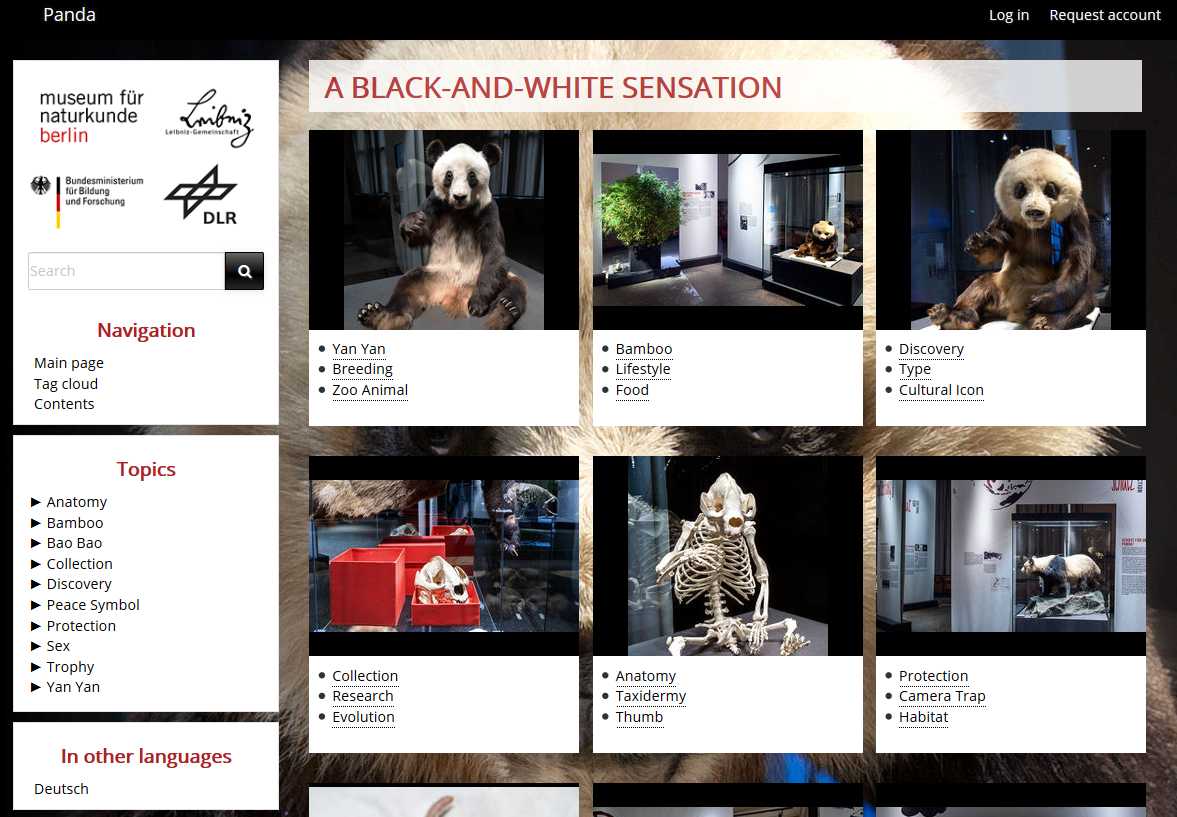
\includegraphics[height=60mm]{panda.png}
    \caption{http://biowikifarm.net/v-mfn/panda}
  \end{figure}
\end{frame}

{\scriptsize
\begin{frame}
  \frametitle{Konkretes Beispiel: das Panda-Wiki\\\textcolor{mfn_green}{A specific example: the Panda wiki}}
  Aus diesen Gründen hat das Museum entschieden, eine Kooperationsumgebung aufzusetzen. Als ich am Museum in 2014 angefangen habe, war mein erster Auftrag mit Wikis zu experimentieren, um eine Kooperationsumgebung zu schaffen. Heutzutage gibt es 24 Wikis am Museum. Hier ist ein Beispiel: das Wiki der Panda Ausstellung. Dieses Wiki ist interessant weil es alle Stadien eines Projektzyklus durchlaufen hat. Während der Planung der Ausstellung wurde das Wiki benutzt, um die Texte der Ausstellung zu schreiben, und um Materialien für das Ausstellungskatalog zu sammeln. Während der Ausstellung (2015), wurde das Wiki veröffentlicht und diente als Ausstellungswebseite. Nach der Ausstellung dient das Wiki als Ausstellungsarchiv. \\
  \bigskip
  \textcolor{mfn_green}{For these reasons, the Museum decided to set up a cooperation environment. When I joined the Museum in 2014, my first job was to experiment with wikis to create such an environment. There are currently 24 wikis at the Museum, here is an example: the wiki of the Panda exhibition. This wiki is interesting because it went through the life-cycle of a whole project: during project planing, it was used to write texts for the labels in the exhibition, and to gather material for the exhibition catalogue. During the exhibition (2015), it was made public and was used as exhibition website. After the exhibition, the wiki can now be used as exhibition archive.}
\end{frame}
}
%----------------------------------------------------------------------------------------------%
% 12. Wikis am Museum
\begin{frame}
  \frametitle{Wikis am Museum / \textcolor{mfn_green}{Wikis at the Museum}}

  \begin{itemize}
  \item{Forschungsprojekte können ein Wiki nutzen, sofern sie es wünschen}
  \item{Wikis sind standardmäßig privat, können aber zum Teil oder im Ganzen geöffnet werden}
  \item{Wikis sind semantisch: sie können sowohl mit Freiformtexten als auch mit strukturierten Daten umgehen}
  \end{itemize}
  
  \begin{itemize}
  \item{\textcolor{mfn_green}{Research projects may use a wiki if they wish to do so}}
  \item{\textcolor{mfn_green}{Wikis are private by default, but may be made public in part or in whole}}
  \item{\textcolor{mfn_green}{Wikis are semantic, so can be used with plain texts as well as with structured data}}
  \end{itemize}
\end{frame}

{\scriptsize
\begin{frame}
  \frametitle{Wikis am Museum / \textcolor{mfn_green}{Wikis at the Museum}}
Forschungsprojekte am Museum können ein Wiki benutzen, wenn sie das wünschen. Obwohl Projekte sehr verschieden sein können, haben die Wikis dennoch gemeinsame Anforderungen. Die Zwei wichtigste Anforderungen sind: die Wikis sind standardmäßig privat. WissenschaftlerInnen sind manchmal abgeneigt, Forschungsergebnisse zu teilen, bevor diese in einer wissenschaftlichen Zeitschrift publiziert worden sind. Die zweite wichtige Anfordeung ist, dass die Wikis semantisch sein sollen. Das heißt, dass unsere Wikis nicht nur mit Freiformtexte umgehen können, sondern auch mit strukturierten Daten. Informationen im Wiki können so auf verschiedene Art und Weise durchsucht werden, was ihre Nützlichkeit steigert.\\
  \bigskip
  \textcolor{mfn_green}{Research projects at the Museum may use a wiki to support collaboration within a team, if they wish to do so. Although projects at the Museum can be of very different kinds, the wikis have some requirements in common. Two important requirements are: wikis are by default private. Scientists are sometimes reluctant to share their data and results before their research has been published in an academic journal. The second important requirement is that wikis should be semantic. This means that our wikis are capable of storing free-form texts, in a similar way than Wikipedia can deal with texts, but can also store structured data. Information in the wiki can then be queried in various ways, and that increases value of the information stored in the wiki.}
\end{frame}
}
%----------------------------------------------------------------------------------------------%
% 13. Die derzeitige Praxis
\begin{frame}
  \frametitle{Die derzeitige Praxis / \textcolor{mfn_green}{The current practice}}
  \begin{figure}
    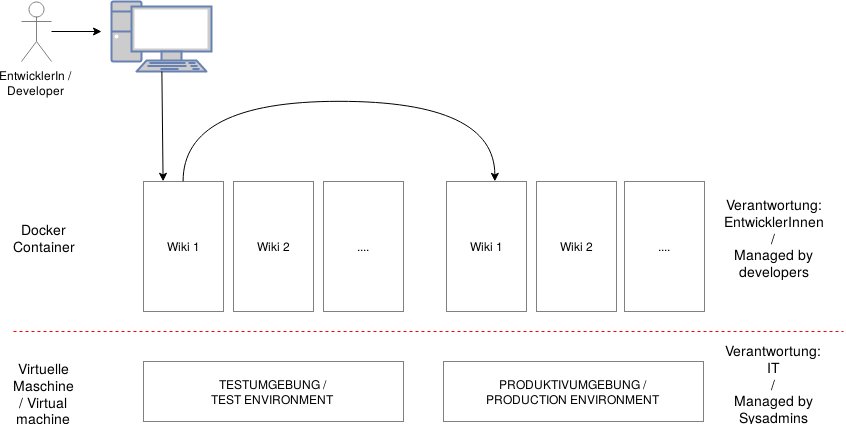
\includegraphics[width=110mm]{docker_wikis.png}
  \end{figure}
\end{frame}

{\scriptsize
\begin{frame}
  \frametitle{Die derzeitige Praxis / \textcolor{mfn_green}{The current practice}}
  Zusammengefasst, um Projekte zu betreiben ist Kooperation gefragt. Kooperation muss von einer Kooperationsumgebung unterstützt werden. Um eine Kooperationsumgebung aufzusetzen werden eine Infrastruktur und Prozesse benötigt. Ich werde die Details des Prozesses in der nächsten Slide zeigen, und auch auf die Probleme eingehen, die dieser Prozesses mit sich bringt. Diese Art von Arbeit hat dennoch ein großes Vorteil: eine deutliche Trennung von den Belangen und Verantwortlichkeiten zwischen EntwicklerInnen und Admins. Admins sind Museumsangestellte, und sie können sich auf das Ausbauen einer Infrastruktur konzentrieren. EntwicklerInnen sind Projektangestellte, manchmal sogar externe Mitarbeiter, und sie können sich darauf konzentrieren, ihr Projekt voranzutreiben.\\
  \bigskip
  \textcolor{mfn_green}{In a nutshell, running projects requires cooperation. Cooperation has to be supported by a cooperation environment. Setting up a cooperation environment requires software infrastructure and processes. I'll go into more detail on the steps of this process on the next slide, and also into the problems this process has. Doing things this way has a very important advantage: a clear separation of concerns and responsibilities between the system administrators and the developers. System administrators are Museum staff, and they can concentrate on building the Museum's infrastructure, which is what they do best. Developers are temporary project staff or external contractors, and they can concentrate on pushing their project forward.}
\end{frame}
}
%----------------------------------------------------------------------------------------------%
% 14. Rolloutprozess
\begin{frame}
  \frametitle{Rolloutprozess / \textcolor{mfn_green}{Roll-out process}}
  \begin{figure}
    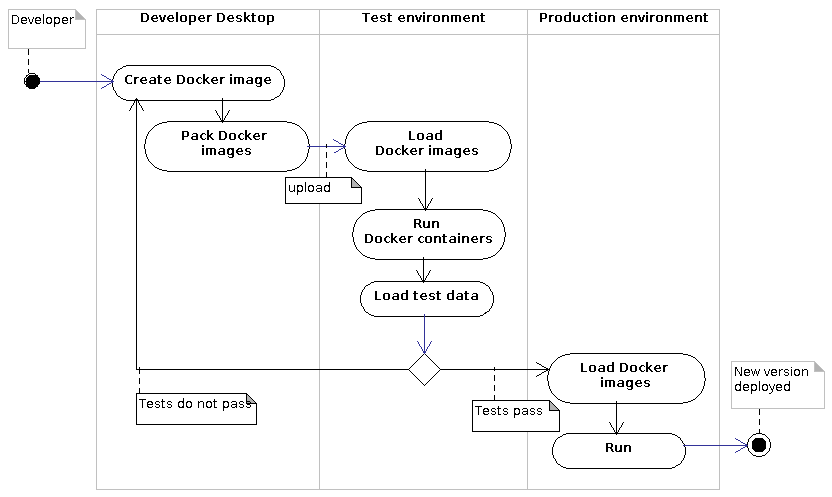
\includegraphics[width=\textwidth]{deploy_wiki_uml.png}
  \end{figure}
\end{frame}

{\scriptsize
\begin{frame}
  \frametitle{Rolloutprozess / \textcolor{mfn_green}{Roll-out process}}
  Das Rollout-Prozess im Detail, so wie es zur Zeit noch implementiert ist. Die derzeitige Praxis am Museum ist, dass Wikis zuerst als Docker Image gebaut werden auf dem Desktop Rechner der EntwicklerInnen. Die Docker Images werden dann auf dem Testserver hochgeladen und getestet. Wenn die Tests bestanden sind, werden die Images auf den Produktivserver eingesetzt.\\
  \bigskip
  \textcolor{mfn_green}{A detailed look at the roll-out process, as it is implemented now. The current practice at the Museum is that new wikis are first build as a Docker image by a developer, at the developers desktop computer. Then the Docker images are uploaded to a test server for testing. If they pass the tests, the images are deployed to the production server.}
\end{frame}
}
%%%%%%%%%%%%%%
%
% The future
%
%%%%%%%%%%%%%%

%----------------------------------------------------------------------------------------------%
% 15. Blick in die Zukunft
\begin{frame}
  \frametitle{Blick in die Zukunft \\ \textcolor{mfn_green}{The shape of things to come}}
  \begin{figure}
    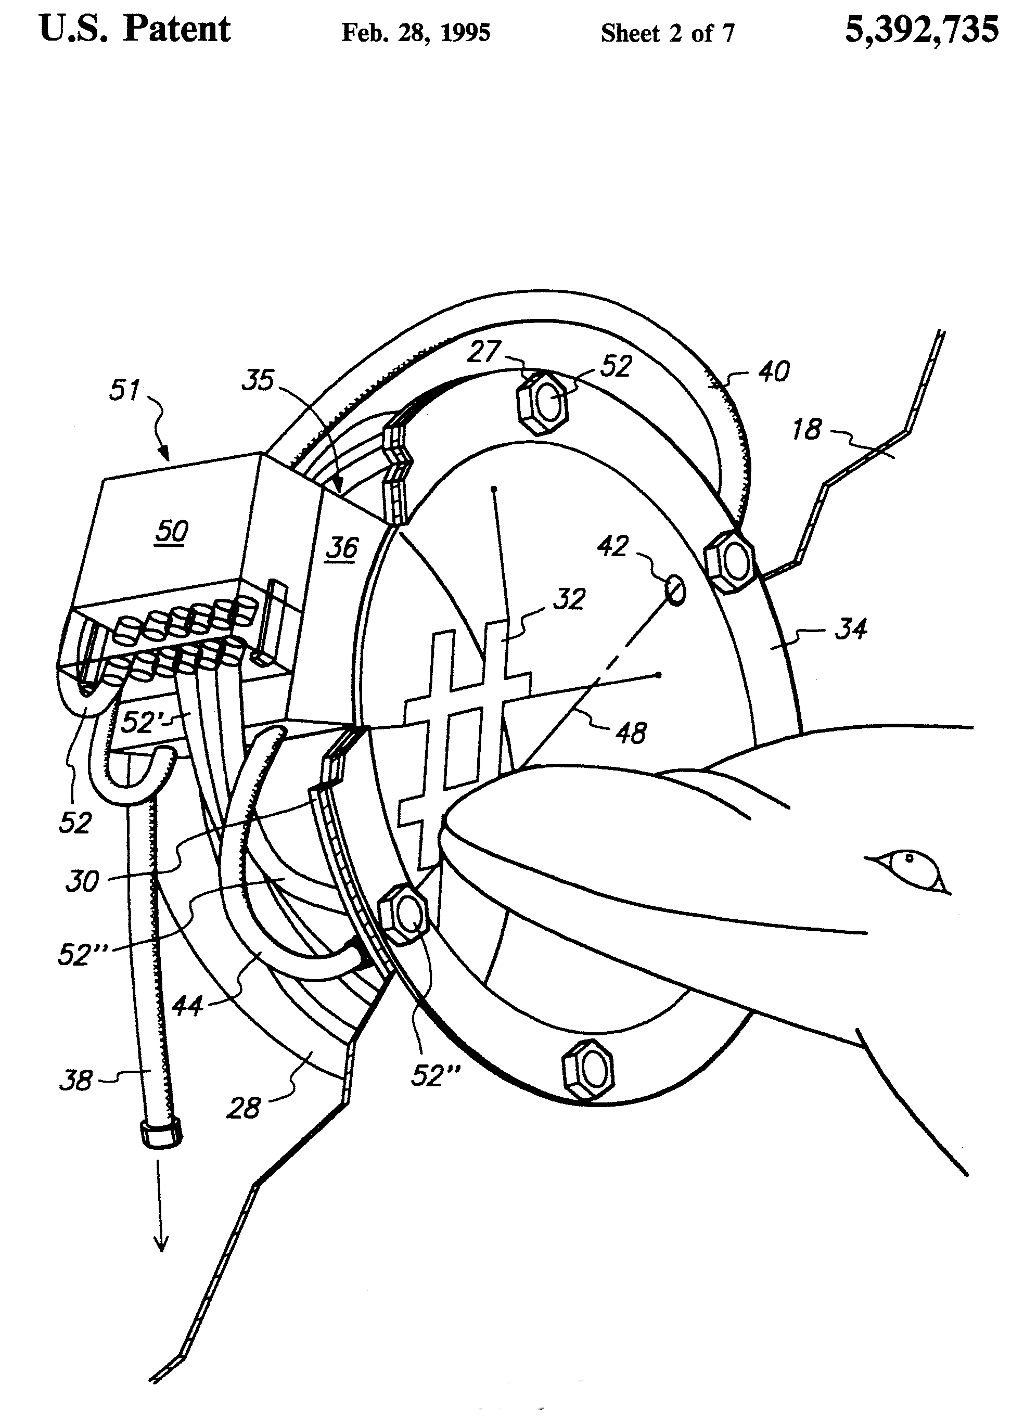
\includegraphics[height=60mm]{marine_mammal_communication.png}
    \caption{Xitco Jr, M.J. et al, 1995. \textit{Marine mammal communication device}. U.S. Patent 5,392,735.}
  \end{figure}
\end{frame}

%----------------------------------------------------------------------------------------------%
% 16. Problemzone
\begin{frame}
  \frametitle{Problemzone / \textcolor{mfn_green}{Problem zone}}
  \begin{figure}
    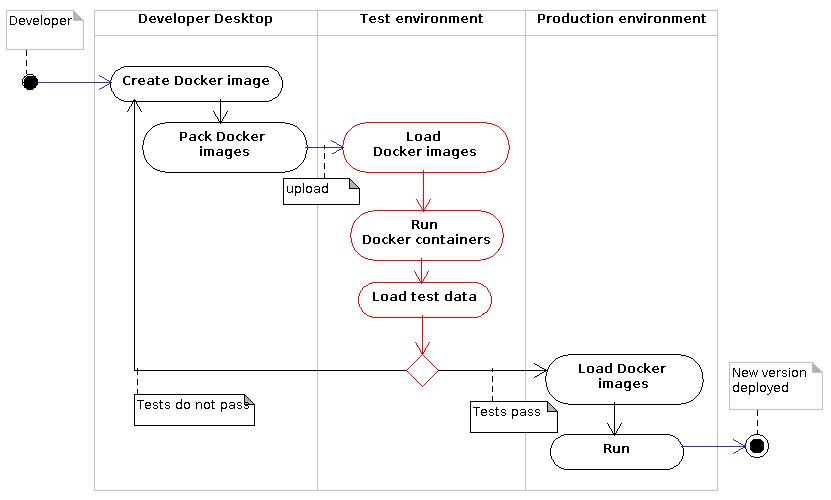
\includegraphics[width=\textwidth]{docker_wikis_problem_uml.png}
  \end{figure}
\end{frame}

{\scriptsize
\begin{frame}
  \frametitle{Problemzone / \textcolor{mfn_green}{Problem zone}}
  Der derzeitige Rollout-Prozess hat offensichtliche Nachteile. Einer davon ist, dass die Testumgebung seht störungsanfällig ist. Da alle Entwickler denselben Server nutzen, ist dieser oft kaputt oder nicht erreichbar. Ein anderes Problem ist, dass viel noch per Hand oder mithilfe von selbsgeschriebenen Skripten gemacht werden muss. Das kostet Zeit und ist nicht besonders pflegefreundlich.\\
  \bigskip
  \textcolor{mfn_green}{As I'm sure some of you have noticed, the current roll-out process has some disadvantages. One is that the test environment is very prone to failure. As all developers use it, it is often broken and unavailable. Another problem is that much of this stuff is done either by hand or through self-written scripts. This takes time and is not easy to maintain.}
\end{frame}
}
%----------------------------------------------------------------------------------------------%
% 17. Lösungsansatz
\begin{frame}
  \frametitle{Lösungsansatz / \textcolor{mfn_green}{Planed solution}}
  \begin{figure}
    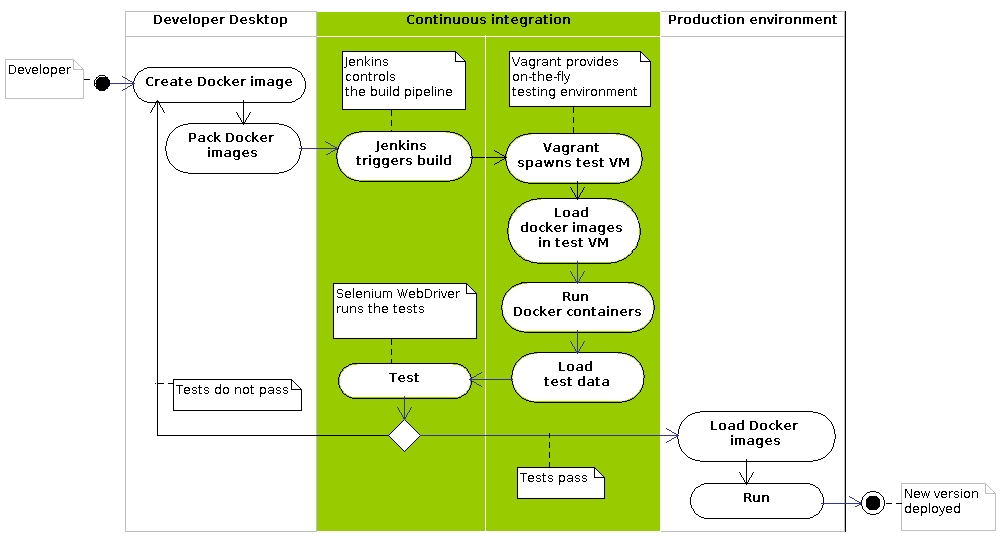
\includegraphics[height=70mm]{docker_wikis_integration.png}
    \caption{\textcolor{mfn_blue}{NOTE: Edited to reflect ideas brought up by Meetup participants.}}
  \end{figure}
\end{frame}

{\scriptsize
\begin{frame}
  \frametitle{Lösungsansatz / \textcolor{mfn_green}{Planed solution}}
  Ich will die Testumgebung durch Continuous Integration ersetzen. Continuous Integration aufzusetzen kann viel Arbeit bedeuten, aber jeder, der damit gearbeitet hat kann bezeugen, dass es sich am Ende lohnt. Continuous Integration automatisiert der Rollout-Prozess, macht testen transparent und wenn es einmal steht, ist sehr einfach zu bedienen. Mein jetziger Plan ist es, um GitLab-CI zu benutzen, um die Continuous Integration Pipeline zu steuern. Test-Werkzeuge und -Data werden in einem Test-Container verpackt. Die Tests können mit Selenium gesteuert weden. Wenn die Tests erfolgreich sind, können die neuen Images in der Produktivumgebung automatisch eingesetzt werden.\\
  \bigskip
  \textcolor{mfn_green}{My current priority is to streamline the roll-out process, by getting rid of the test environment and replacing it with continuous integration. Setting up continuous integration can be a lot of effort, but as anyone who has worked with continuous integration can tell, it is effort well spent. Continuous integration automates the roll-out process, renders testing more transparent, and once it is set up, it is just a mater of submit-and-forget. I am currently planing to use GitLab-CI to build the continuous integration pipeline. Test tools and data will be provided by a test container. The tests can then run in Selenium. If the tests pass, the new images would be deployed to the production environment.}
\end{frame}
}
%----------------------------------------------------------------------------------------------%
% 18. Kontaktdaten
\begin{frame}
  \frametitle{Kontaktdaten / \textcolor{mfn_green}{Contact information}}
  \begin{center}
    Alvaro Ortiz-Troncoso \\
    \medskip
    Email: Alvaro.OrtizTroncoso@mfn.berlin \\    
    \medskip
    Web: https://github.com/MfN-Berlin
  \end{center}
\end{frame}

\end{document}


